\chapter{Pruebas de integración y fiabilidad}

El eje fundamental de este capítulo es mostrar el rendimiento del sistema en diferentes circunstancias, y probar que el mismo es capaz de desenvolverse de forma satisfactoria en la mayoría de escenarios posibles.

\section{Rendimiento del algoritmo de OCR en diferente hardware}

 {
  \huge creo que quedaria mejor al final del cap3
 }

Esta prueba consistió en correr el algoritmo de OCR en diferente hardware y medir el tiempo que tardaba en procesar las imágenes, para ello se armó un dataset con 100 fotografías de vehículos y se las procesaron midiendo el tiempo (Tab. \ref{tab:hardware-test-tiempo}).

\begin{table}
    \centering
    \caption{Pruebas del algoritmo de OCR en diferentes hardware.}
    \label{tab:hardware-test-tiempo}
\end{table}

\section{Prueba de exterior}

Esta prueba se realizó con una cámara Kanon [Incluir data de la camara, es del santi] en el estacionamiento de Ingeniería de la Universidad Nacional del Comahue entre las 8 y 9 de la mañana, el martes 6 de junio del 2023. La prueba se realizó colocando la cámara en un trípode con una altura de 70cm respecto del suelo, y se procedió a filmar los vehículos que entraban en el estacionamiento o pasaban por la calle. De este proceso de medición se obtuvieron dos videos de una duración aproximada de 40min.

Teniendo en cuenta que el algoritmo de OCR tarda 1200ms en procesar un frame es necesario realizar un filtrado, ya que los 40min de filmación equivalen en 72000 imágenes, y la mayoría no poseen vehículos o la patente no está enfocada. El proceso de filtrado consistió en un recorte manual de las partes donde no había ningún vehículo, lo que termino dejando 7min de filmación, si bien este número es bajo llevo a obtener un total de 35 vehículos, suficientes para este análisis. Posteriormente se convirtió el video en frames, utilizando Open CV, para luego procesar las 11000 fotografías y eliminar las que no era posible reconocer la patente del vehículo. Luego se obtuvieron 3600 fotografías válidas, las cuales se procesaron por el algoritmo de OCR y se descartaron todas las imágenes que tenían un porcentaje de seguridad inferior al $50\%$, las imágenes se clasificaron se guardando en una carpeta con el valor predicho por el algoritmo.
Finalmente se contabilizaron los errores generando el resumen de Tab. \ref{tab:resumen-patente}.

\begin{table}
    \centering
    \begin{tabular}{cccccccc}
    \toprule
    Caracteres & Perfectas & 1 error & 2 errores & 3 errores & 4 errores & 5 errores & $\sum$ \\
    \midrule
    6          & 60        & 78      & 25        & 10        & 3         & 0         & 176    \\
    7          & 282       & 185     & 49        & 5         & 1         & 1         & 523    \\
    $\sum$     & 342       & 263     & 74        & 15        & 4         & 1         & 699    \\
    \bottomrule
\end{tabular}

    \caption{Resumen de las patentes reconocidas.}
    \label{tab:resumen-patente}
\end{table}

\subsection{Análisis de resultados}

De esta prueba se observa que el rendimiento del algoritmo ronda los $49\%$ de aciertos, que se considera bajo, sin embargo cabe destacar que no se detuvo a los vehículos para captar la fotografías. La cual no es el entorno de trabajo del sistema, por lo que se puede decir que el funcionamiento debería ser mejor.

\section{Pruebas de distancia y ángulo}

Para realizar esta serie de pruebas se colocó un Volkswagen Up modelo 2015 con patente PEY232 en una posición fija, se procedió a medir con una cinta métrica de error 1cm. El ángulo de $0^\circ$ corresponde al centro de la patente, mientras que el origen se tomó desde el inicio desde la finalización de la patente, en Fig. \ref{fig:sistema-medicion-angulos} se puede apreciar un esquema del sistema de ejes. La medición para una distancia y ángulo se realizó capturando una fotografía con la cámara de los sistemas SL para luego procesarla por el algoritmo de OCR. Las distancias utilizadas fueron desde 50cm hasta 3m con un paso de 50cm (Tab. \ref{tab:resumen-distancia}). Por otro lado los ángulos elegidos fueron desde $-60^\circ$ hasta $60^\circ$ con un paso de $30^\circ$, dando como resultados la Tab. \ref{tab:resumen-angulo}, en la Fig. \ref{fig:fotos-angulo} se observan las fotos.

\begin{figure}
    \centering
    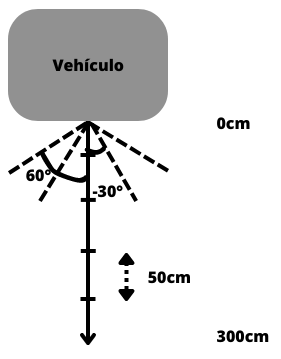
\includegraphics[width=.3\textwidth]{imgs/sistema-referencia.png}
    \caption{Sistema de referencia.}
    \label{fig:sistema-medicion-angulos}
\end{figure}

\begin{table}
    \centering
    \begin{tabular}{rl}
    \toprule
    Distancia & Predicción \\
    \midrule
    50        & PEY232     \\
    100       & PEY232     \\
    150       & PEY232     \\
    200       & PEY232     \\
    250       & PEY232     \\
    300       & PEY232     \\
    \bottomrule
\end{tabular}

    \caption{Resumen de la prueba de distancia.}
    \label{tab:resumen-distancia}
\end{table}

\begin{table}
    \centering
    \begin{tabular}{rl}
    \toprule
    Ángulo & Predicción \\
    \midrule
    -60    & PEY232     \\
    -30    & PEY232     \\
    0      & PEY232     \\
    30     & PEY232     \\
    60     & PEY232     \\
    \bottomrule
\end{tabular}

    \caption{Resumen de la prueba de ángulos.}
    \label{tab:resumen-angulo}
\end{table}

\begin{figure}
    \centering
    \begin{subfigure}{.3\textwidth}
        \centering
        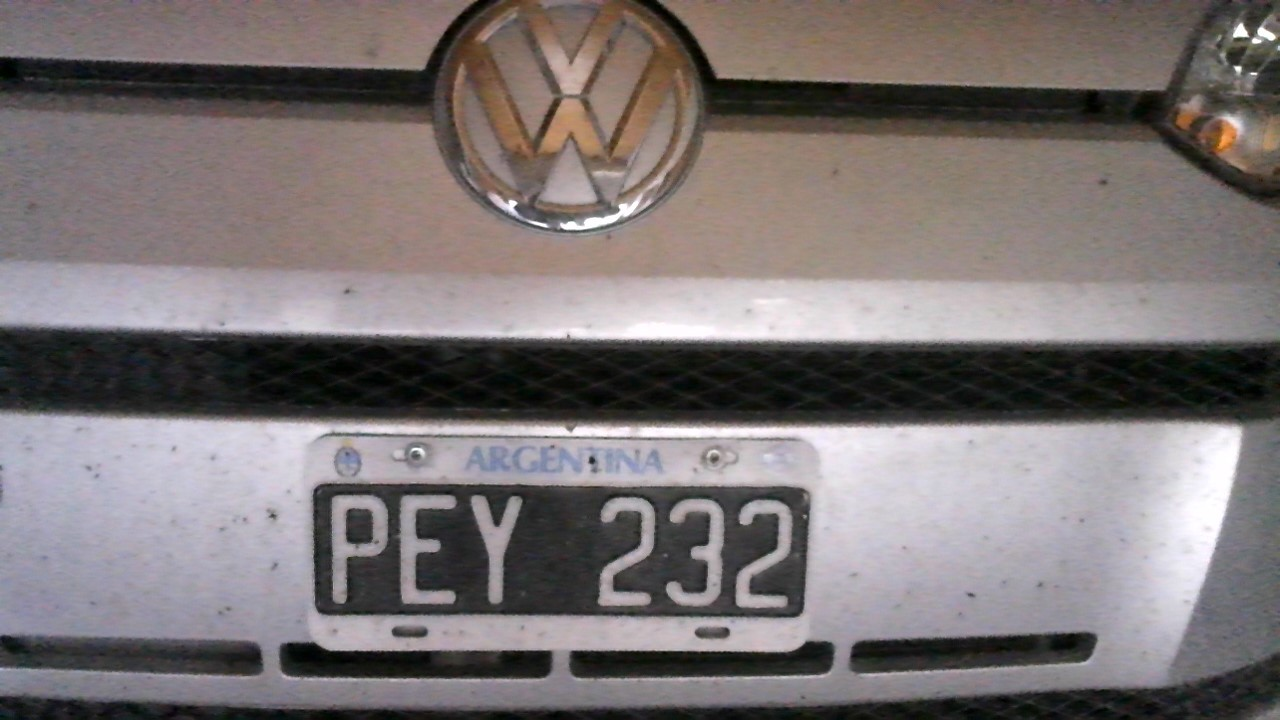
\includegraphics[width=\textwidth]{imgs/test-distancia/0_50.jpg}
        \caption{50cm}
    \end{subfigure}
    \begin{subfigure}{.3\textwidth}
        \centering
        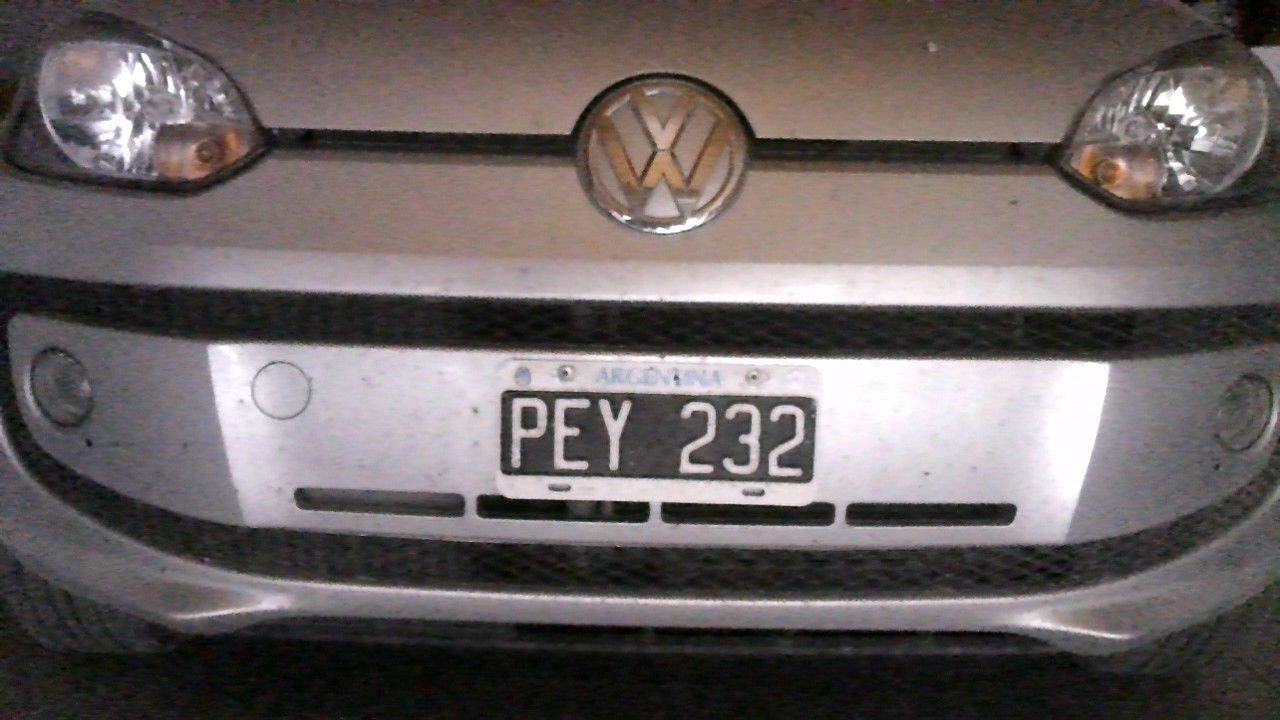
\includegraphics[width=\textwidth]{imgs/test-distancia/0_100.jpg}
        \caption{100cm}
    \end{subfigure}
    \begin{subfigure}{.3\textwidth}
        \centering
        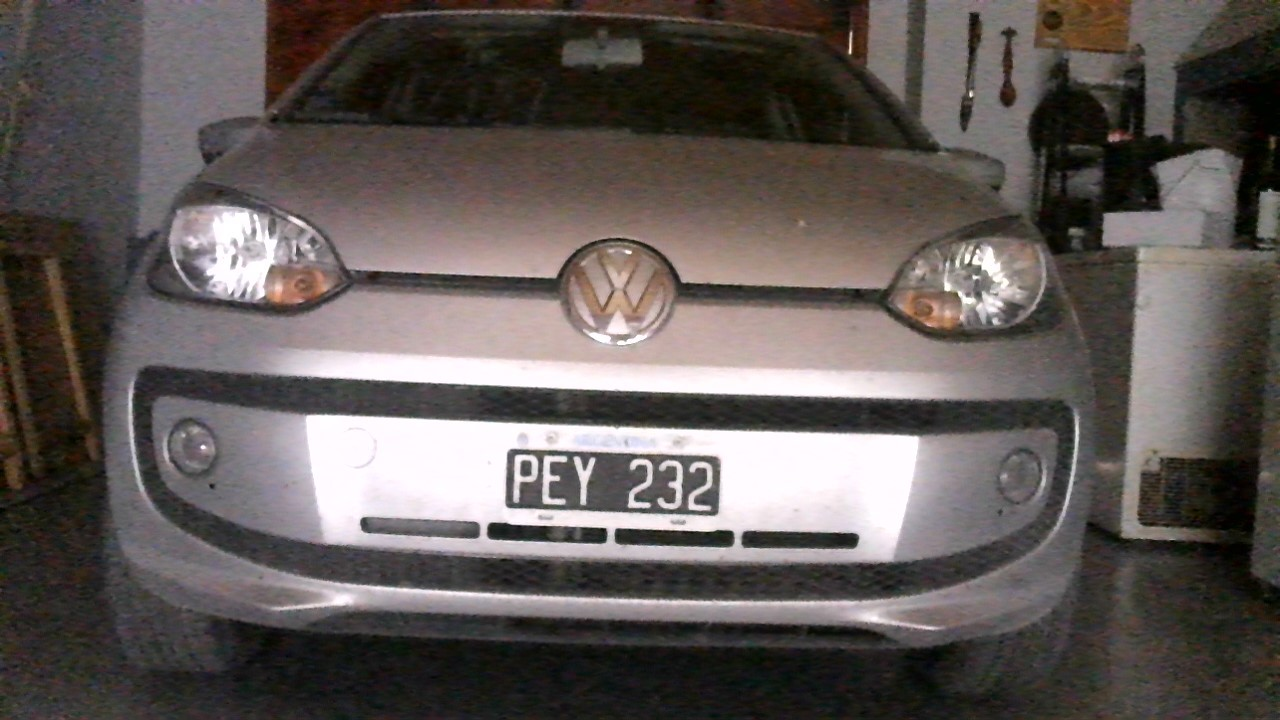
\includegraphics[width=\textwidth]{imgs/test-distancia/0_150.jpg}
        \caption{150cm}
    \end{subfigure}
    \begin{subfigure}{.3\textwidth}
        \centering
        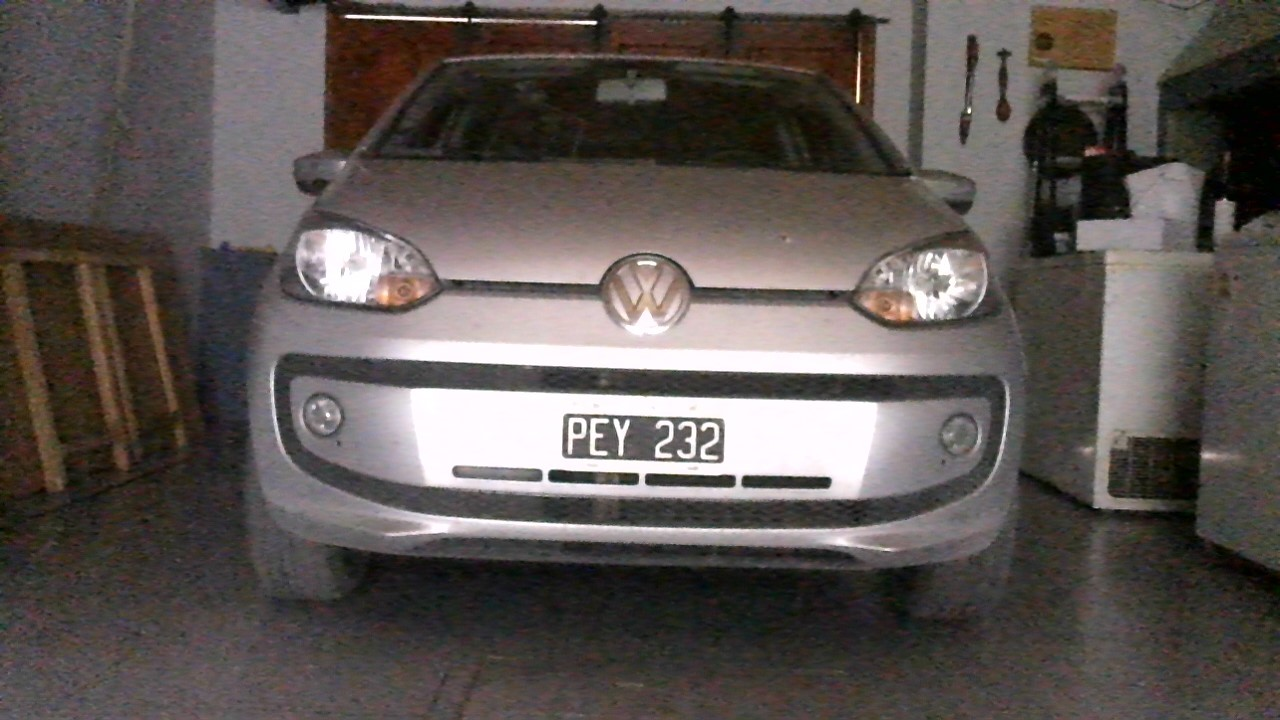
\includegraphics[width=\textwidth]{imgs/test-distancia/0_200.jpg}
        \caption{200cm}
    \end{subfigure}
    \begin{subfigure}{.3\textwidth}
        \centering
        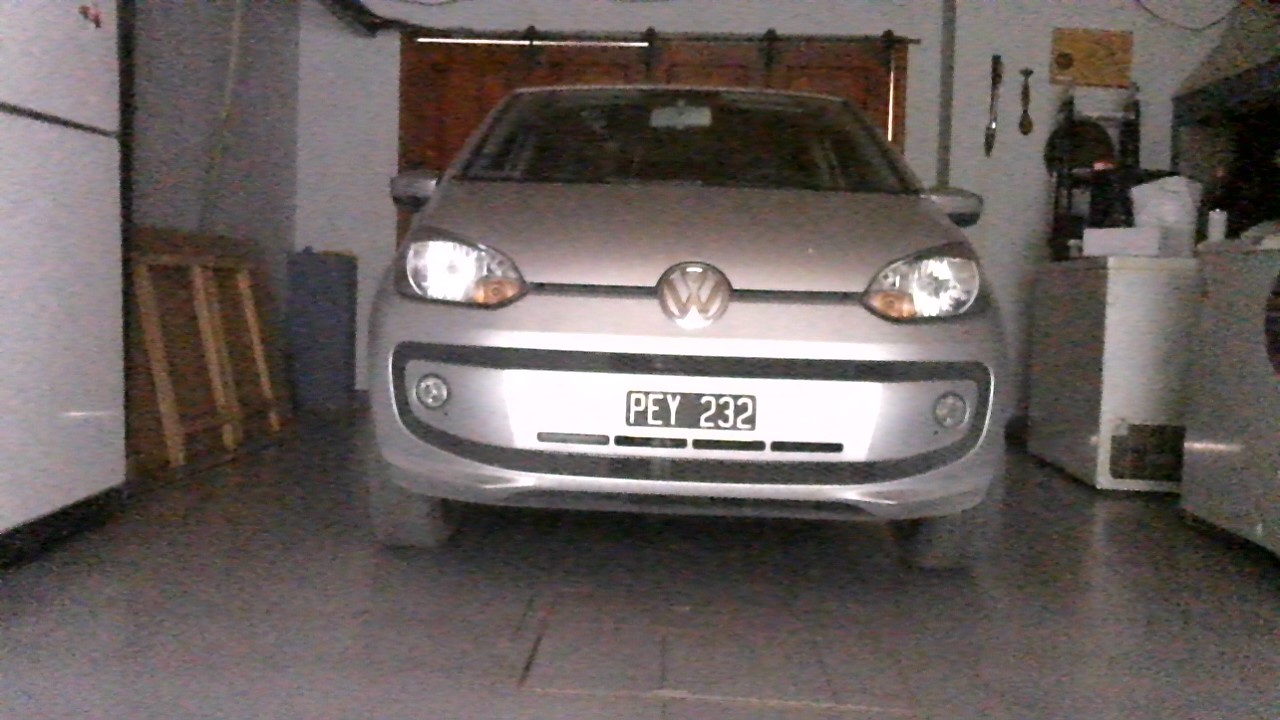
\includegraphics[width=\textwidth]{imgs/test-distancia/0_250.jpg}
        \caption{250cm}
    \end{subfigure}
    \begin{subfigure}{.3\textwidth}
        \centering
        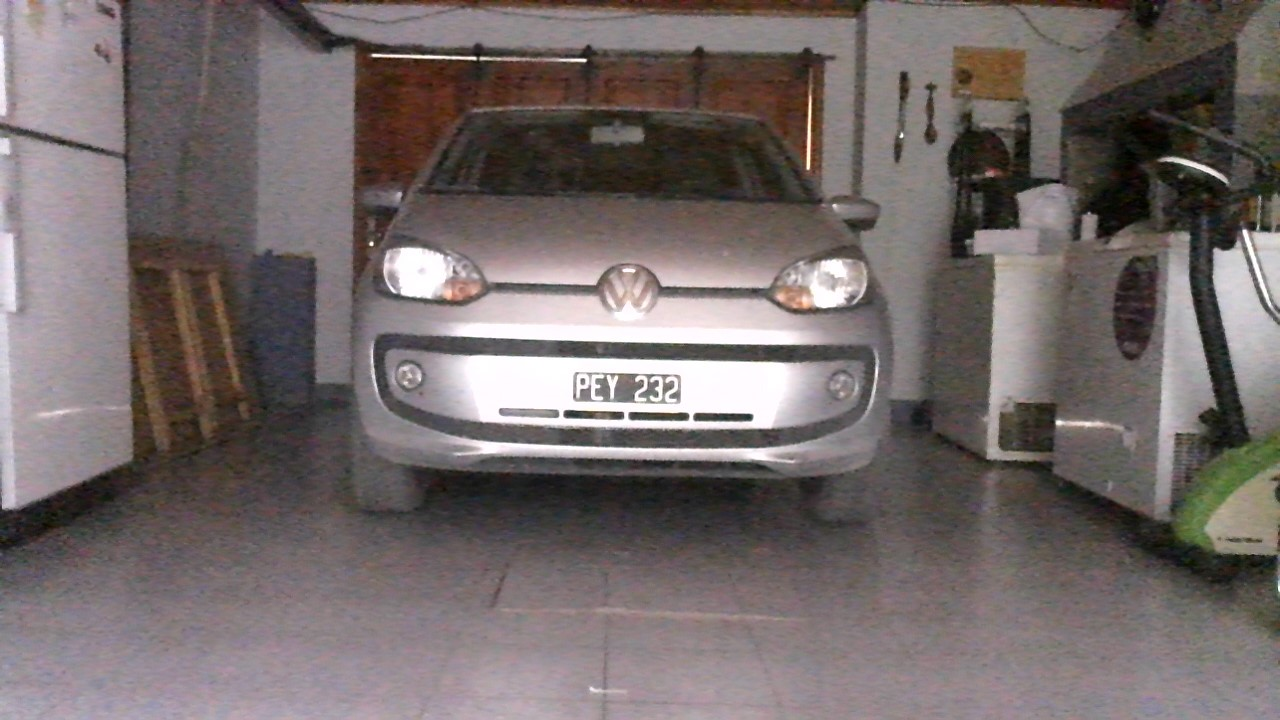
\includegraphics[width=\textwidth]{imgs/test-distancia/0_300.jpg}
        \caption{300cm}
    \end{subfigure}
    \caption{Fotografías a diferentes distancias.}
    \label{fig:fotos-distancia}
\end{figure}

\begin{figure}
    \centering
    \begin{subfigure}{.15\textwidth}
        \centering
        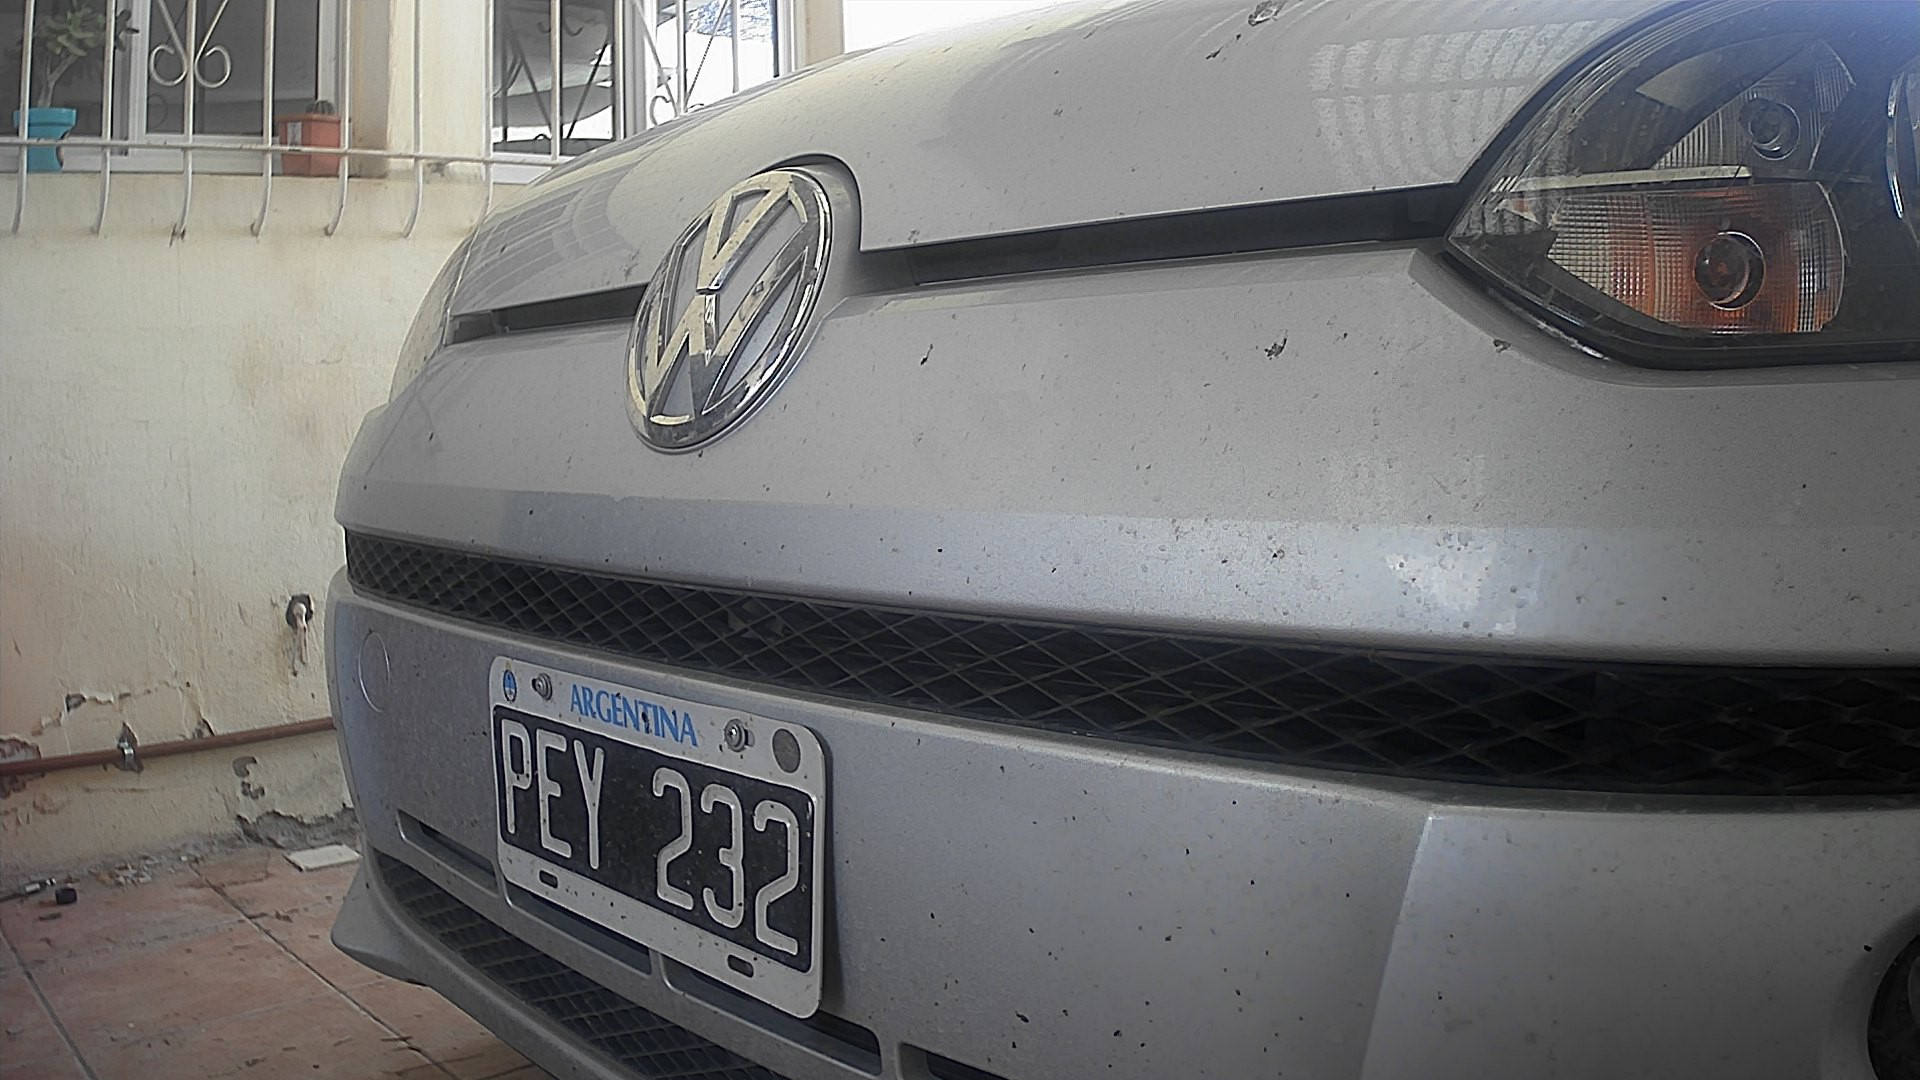
\includegraphics[width=\textwidth]{imgs/test-angulos/-60_50.jpg}
        \caption{$-60^\circ$}
    \end{subfigure}
    \begin{subfigure}{.15\textwidth}
        \centering
        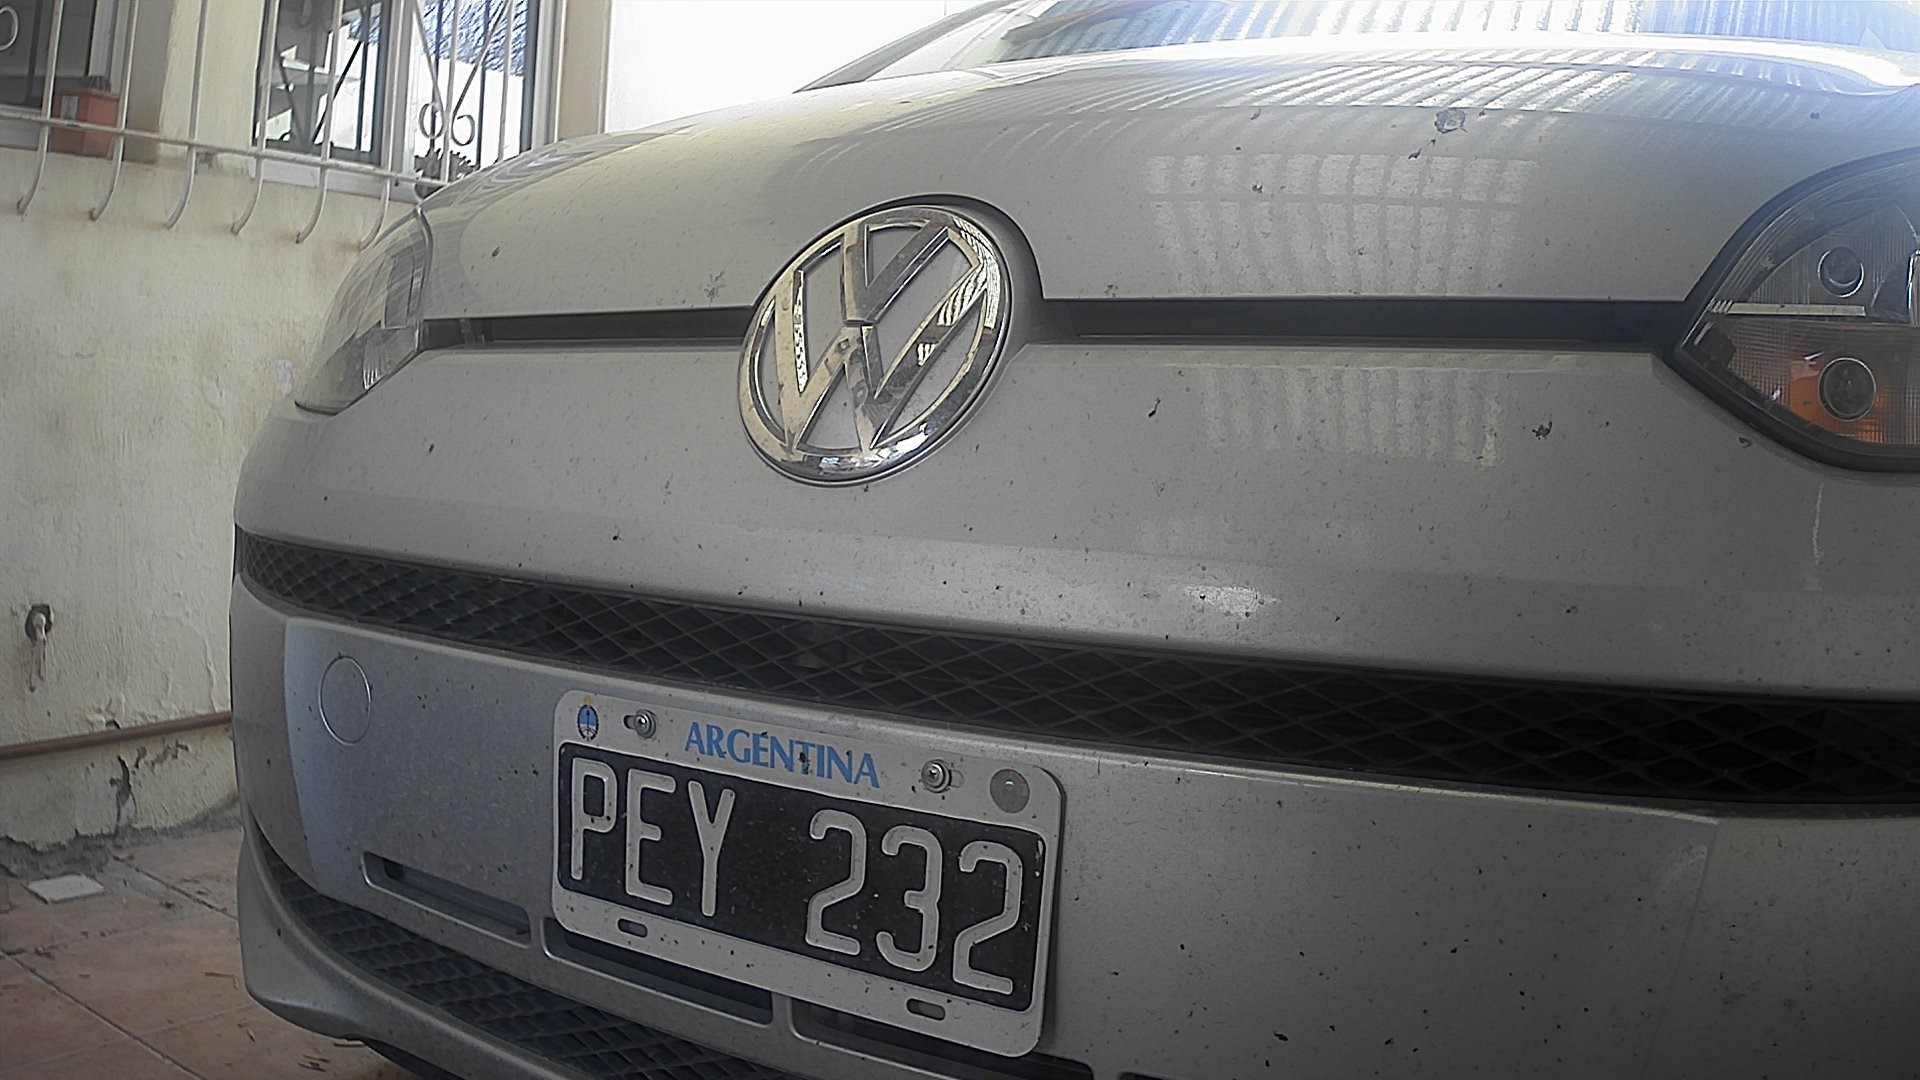
\includegraphics[width=\textwidth]{imgs/test-angulos/-30_50.jpg}
        \caption{$-30^\circ$}
    \end{subfigure}
    \begin{subfigure}{.15\textwidth}
        \centering
        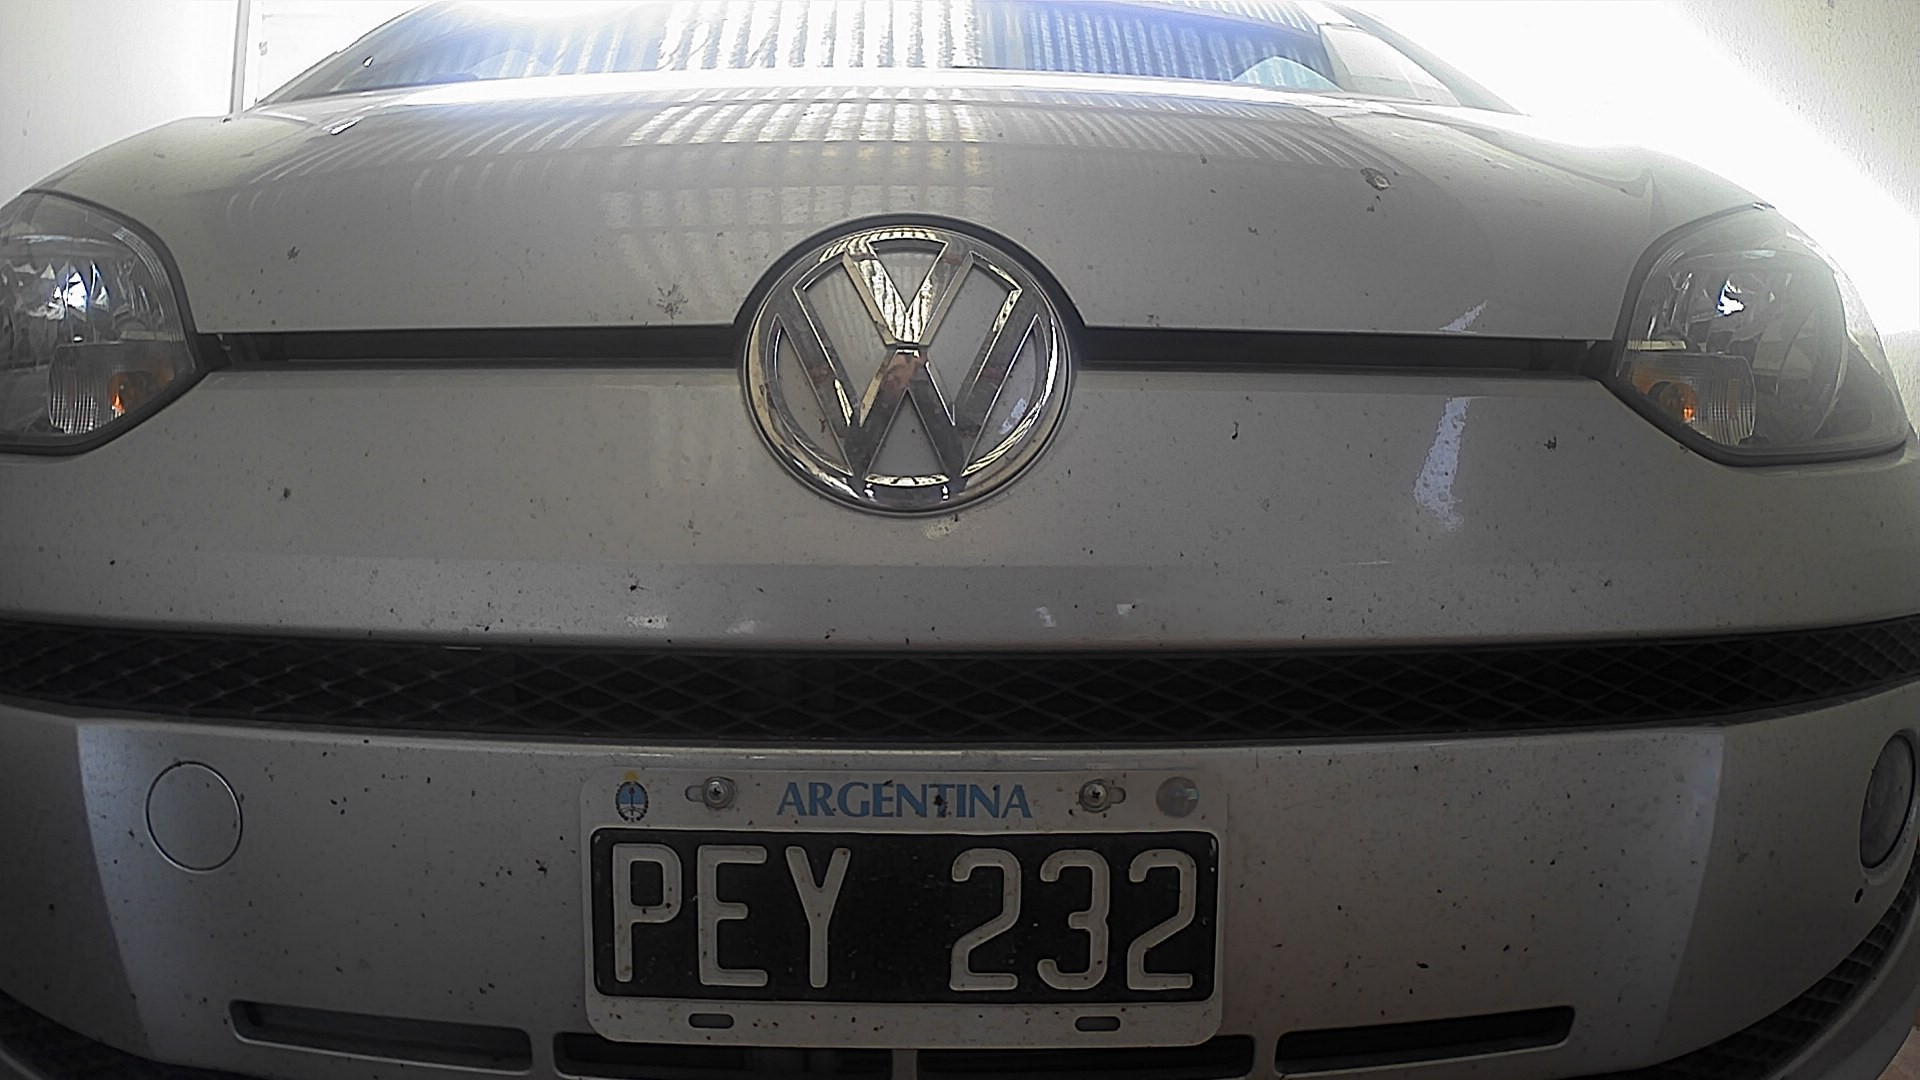
\includegraphics[width=\textwidth]{imgs/test-angulos/0_50.jpg}
        \caption{$0^\circ$}
    \end{subfigure}
    \begin{subfigure}{.15\textwidth}
        \centering
        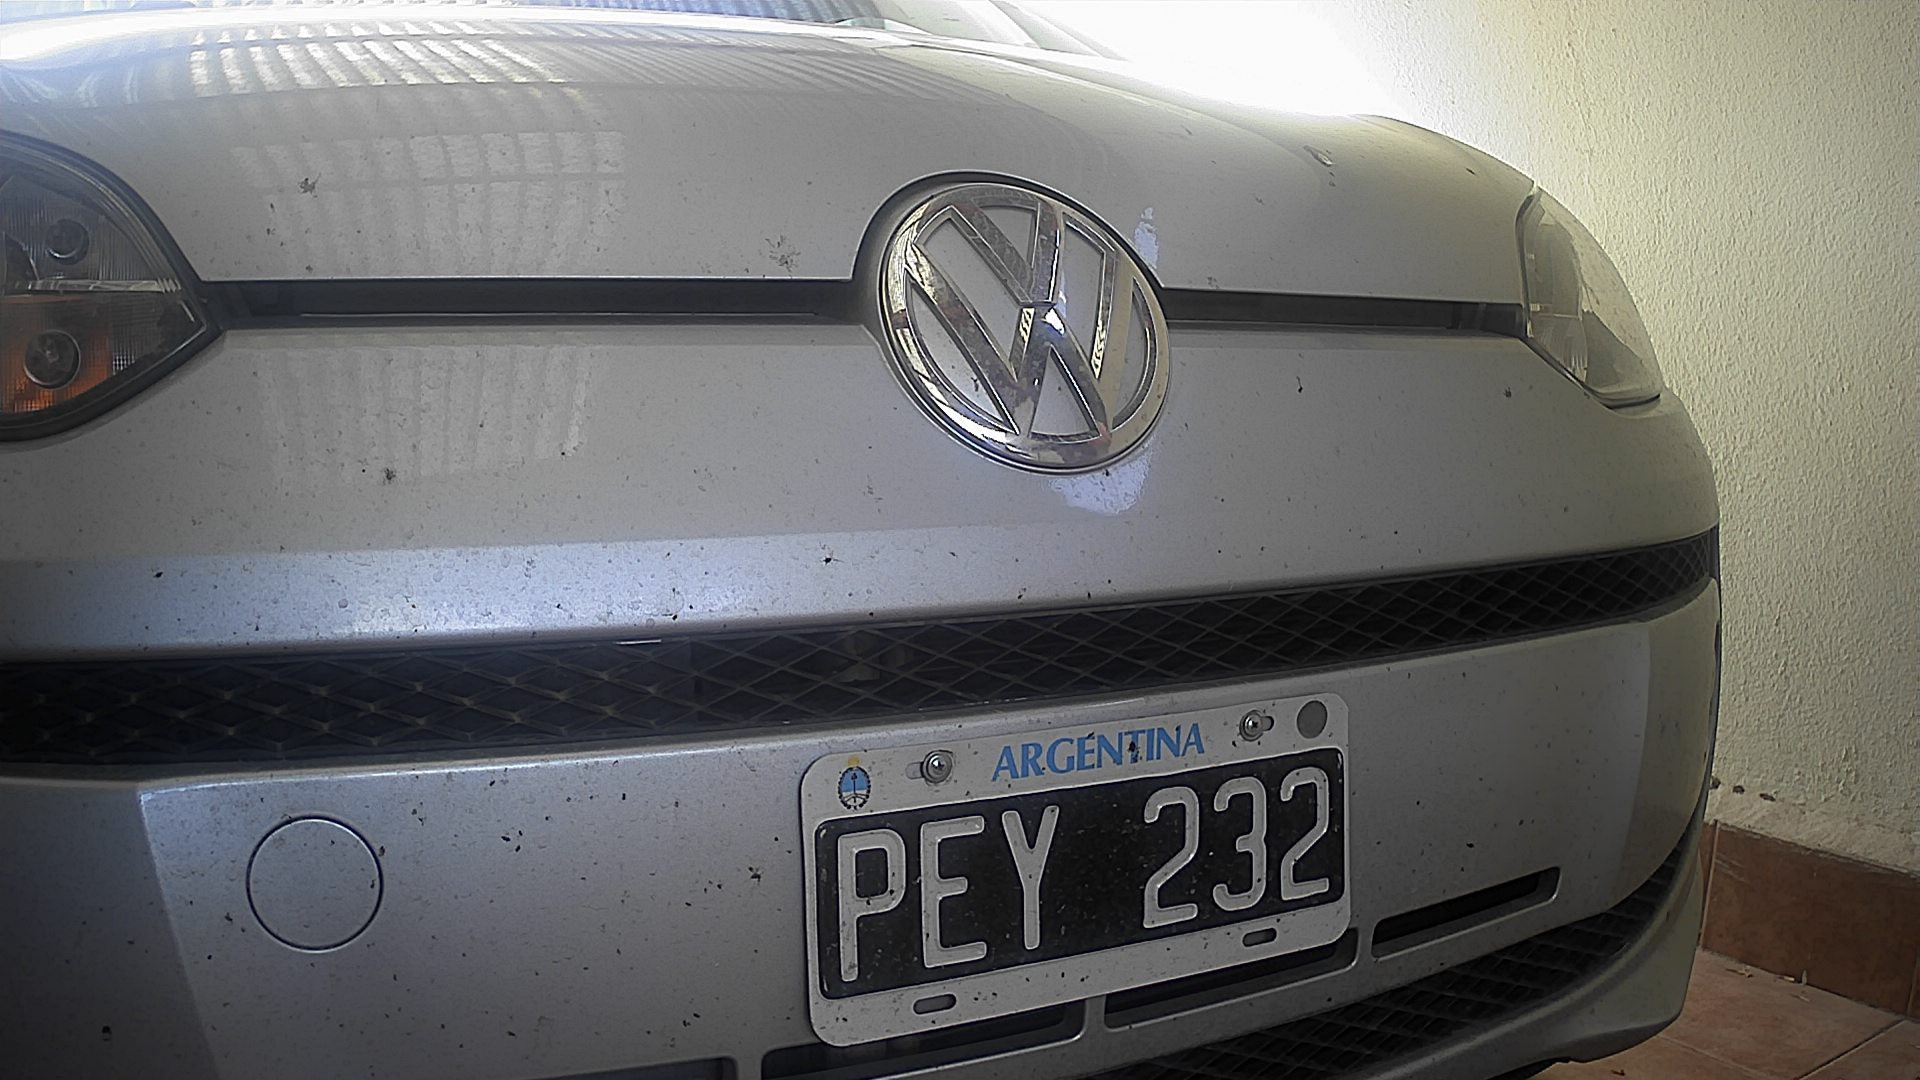
\includegraphics[width=\textwidth]{imgs/test-angulos/30_50.jpg}
        \caption{$30^\circ$}
    \end{subfigure}
    \begin{subfigure}{.15\textwidth}
        \centering
        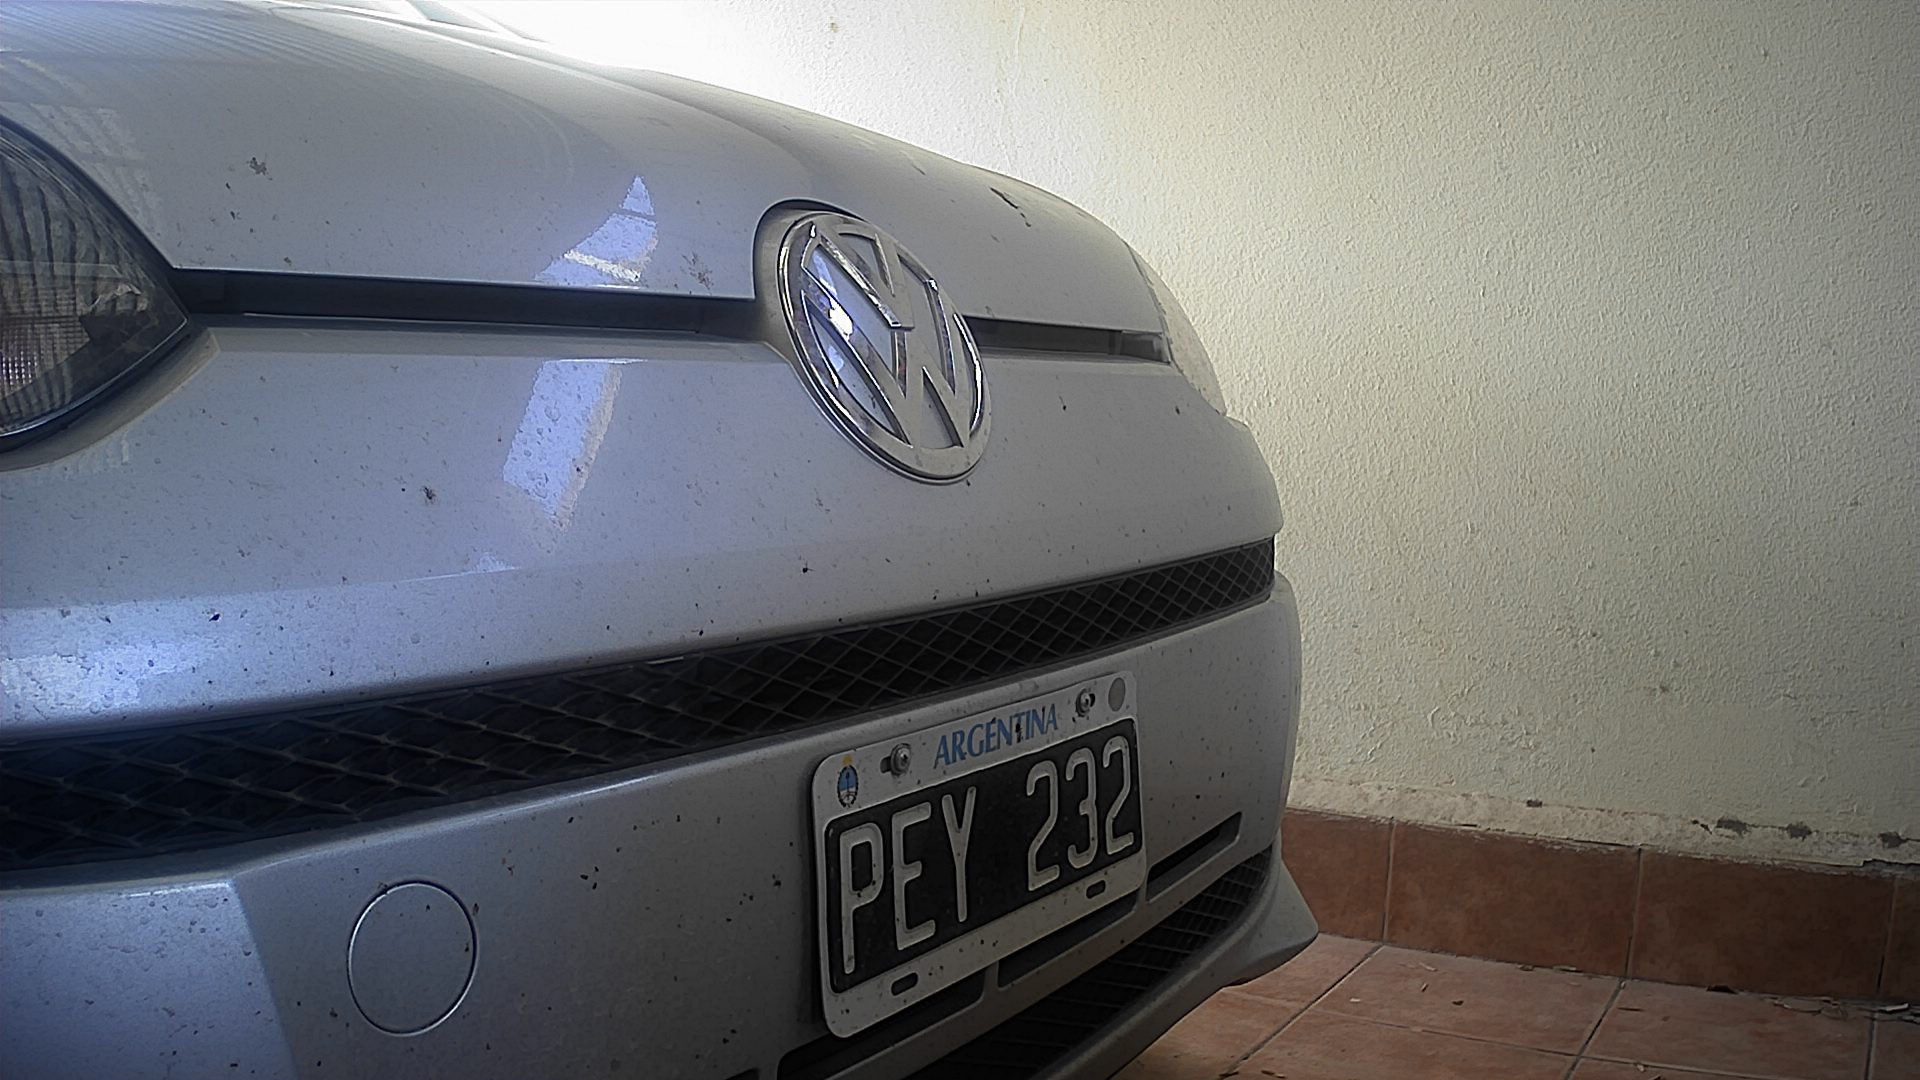
\includegraphics[width=\textwidth]{imgs/test-angulos/60_50.jpg}
        \caption{$60^\circ$}
    \end{subfigure}
    \caption{Fotografías a diferentes ángulos.}
    \label{fig:fotos-angulo}
\end{figure}

\subsection{Análisis de resultados}

Con esta prueba se logró probar el sistema en diferentes distancias y ángulos obteniendo un resultado satisfactorio en todas las pruebas, probando que el sistema funciona de forma correcta en un entorno controlado.

\section{Pruebas sobre el servidor}

\subsection{Integración sistema SL y servidor}

Se montó un sistema SL junto con una notebook como servidor [fig del garage con el auto] y se crearon registros de entrada, y cambiando la configuración en tiempo real. Con esta prueba se logró probar los cambios de configuración en tiempo real y que los registros se creen de forma correcta.

\subsection{Creación de registros}

Para probar el correcto de funcionamiento del servidor, se creó un usuario de admin y un cliente. Se crearon 2 lugares junto con un script en Python 3 emulando el envío de datos de las barreras, generando el servidor 5900 registros para los lugares, probando el funcionamiento del sistema de inicio a fin.




